\documentclass[11pt]{preprint}

\setlength{\topmargin}{0mm} \setlength{\oddsidemargin}{0mm}
\setlength{\textwidth}{160mm} \setlength{\textheight}{215mm}

\usepackage{amssymb,amsmath,amscd,amsthm}
\usepackage{tikz}

\newtheorem{proposition}{Proposition}

\def\enumb{\begin{enumerate}}
\def\enume{\end{enumerate}}
\def\integers{\mathbb{Z}}
\def\multiset#1#2{\ensuremath{\left(\kern-.3em\left(\genfrac{}{}{0pt}{}{#1}{#2}\right)\kern-.3em\right)}}

\title{Discrete Mathematics, 2016 Spring - HW 5}
\author{Instructor: Zsolt Pajor-Gyulai}
\institute{Courant Institute of Mathematical Sciences, NYU}



\begin{document}

\maketitle

To get full credit  in all of the problems, use rigorous justification and unless otherwise indicated, make sure that your solution reads as a perfect English sentence. You should only assume integers, operations and order relations as given. If you use a statement or a definition from the textbook, make sure to indicate it.
\vspace{0.2cm}

\textbf{Section 17}
\enumb
%\item[6)]
%\enumb
%\item How many $n$-digit binary $(0,1)$ sequences contain exactly $k$ 1s?
%\item How many $n$-digit ternary $(0,1,2)$ sequences contain exactly $k$ 1s?
%\enume

\item[8)] Fifty runners compete in a $10K$ race. How many outcomes are possible if
\enumb
\item We want to know in what place every runner finished.
\item The race is a qualifying race and we just want to pick the 10 fastest runners.
\item The race is an Olympic final event, and we care only about who gets the gold, silver, and bronze medals.
\enume
\item[17)] Let $n\geq k\geq m\geq 0$ be integers. Consider the following formula:
\[
\binom{n}{k}\binom{k}{m}=\binom{n}{m}\binom{n-m}{k-m}
\]
Give two different proofs. One proof should use the factorial formula, the other should be combinatorial.
\item[30)] 
\enumb
\item What is the coefficient of $x^3y^5$ in $(x+y+4)^{10}$?
\item Prove that $\binom{n}{a~b~c}=\binom{n}{a}\binom{n-a}{b}$. Here $a,b,c$ are natural numbers with $a+b+c=n$.
\enume

%\item[32-33)] A poker hand consits of $5$ cards chosen from a standard deck of $52$ cards. 
%\enumb
%\item How many different poker hands are possible?
%\item How many hands are a four of a kind?
%\item ...three of a kind?
%\item ...Flush?
%\item ...Full house?
%\item ...Straight?
%\item ...Straight flush?
%\enume
\enume

\textbf{Section 18}
\enumb
\item[8)] Express $\multiset{n}{k}$ using factorial notation.
\item[N/A)] $8$ identical prizes are given out to chosen students in a class of size $32$.
\enumb
\item How many ways can this be done if one student can only get one prize?
\item How many ways can this be done if any student can get any number of prizes?
\enume 
\item[7,11)]
\enumb
\item Calculate $\multiset{8}{4}$ and $\multiset{4}{8}$. Notice anything interesting?
\item Show that for any positive integer $a$, 
\[
\multiset{2a}{a}=2\multiset{a}{2a}.
\]
\enume
\enume

\textbf{Section 19}

\enumb
\item[3)] How many integers between $1$ and $1,000,000$ (inclusive) are not divisible by $2$, $3$, or $5$?
\item[8)] How many lattice paths through the grid in the figure avoids both locations $A$ and $B$?
\begin{figure}[h]
\centering
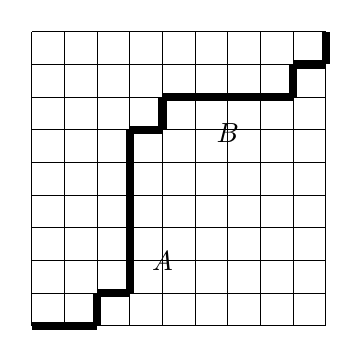
\begin{tikzpicture}[scale=0.415]
\foreach \i in {0,1,2,3,4,5,6,7,8,9}
	{
		\draw (\i,0) -- (\i,9);
	}
	
\foreach \i in {0,1,2,3,4,5,6,7,8,9}
	{
		\draw (0,\i) -- (9,\i);
	}
	
\draw[line width=3pt] (0,0) -- (2,0);
\draw[line width=3pt] (2,0) -- (2,1);
\draw[line width=3pt] (2,1) -- (3,1);
\draw[line width=3pt] (3,1) -- (3,6);
\draw[line width=3pt] (3,6) -- (4,6);
\draw[line width=3pt] (4,6) -- (4,7);
\draw[line width=3pt] (4,7) -- (8,7);
\draw[line width=3pt] (8,7) -- (8,8);
\draw[line width=3pt] (8,8) -- (9,8);
\draw[line width=3pt] (9,8) -- (9,9);


\node at (4,2) {$A$};
\node at (6,5.9) {$B$};

\end{tikzpicture}
\end{figure}
\enume
\end{document}